\section{实验结果与分析}
\label{sec:results}

本章从分类精度、计算效率、预训练增益、大语言模型表现以及精度-效率权衡五个角度分析实验结果。所有数据均在第~\ref{sec:experiment}~节所述的统一实验设置下运行一次获得。

\subsection{整体性能对比}
\label{sec:overall_performance}

五模型在测试集上的综合性能如表~\ref{tab:all_results}、图~\ref{fig:perf} 与雷达图~\ref{fig:radar} 所示。

\begin{table}[htbp]
    \centering
    \caption{五模型整体性能对比}
    \label{tab:all_results}
    \begin{tabular}{lcccc}
        \toprule
        模型 & Accuracy & Precision & Recall & F1-Score \\
        \midrule
        SVM + TF-IDF     & 0.8933 & 0.8974 & 0.8914 & 0.8944 \\
        Bi-LSTM          & 0.8983 & 0.8945 & 0.9062 & 0.9003 \\
        BERT (Fine-tune) & 0.9517 & 0.9568 & 0.9474 & 0.9521 \\
        Qwen-7B (Zero)   & 0.9000 & 0.851 & 0.8734 & 0.8985 \\
        Qwen-7B (LoRA)   & \textbf{0.9567} & \textbf{0.9633} & \textbf{0.9507} & \textbf{0.9570} \\
        \bottomrule
    \end{tabular}
\end{table}

\begin{figure}[h!]
    \centering
    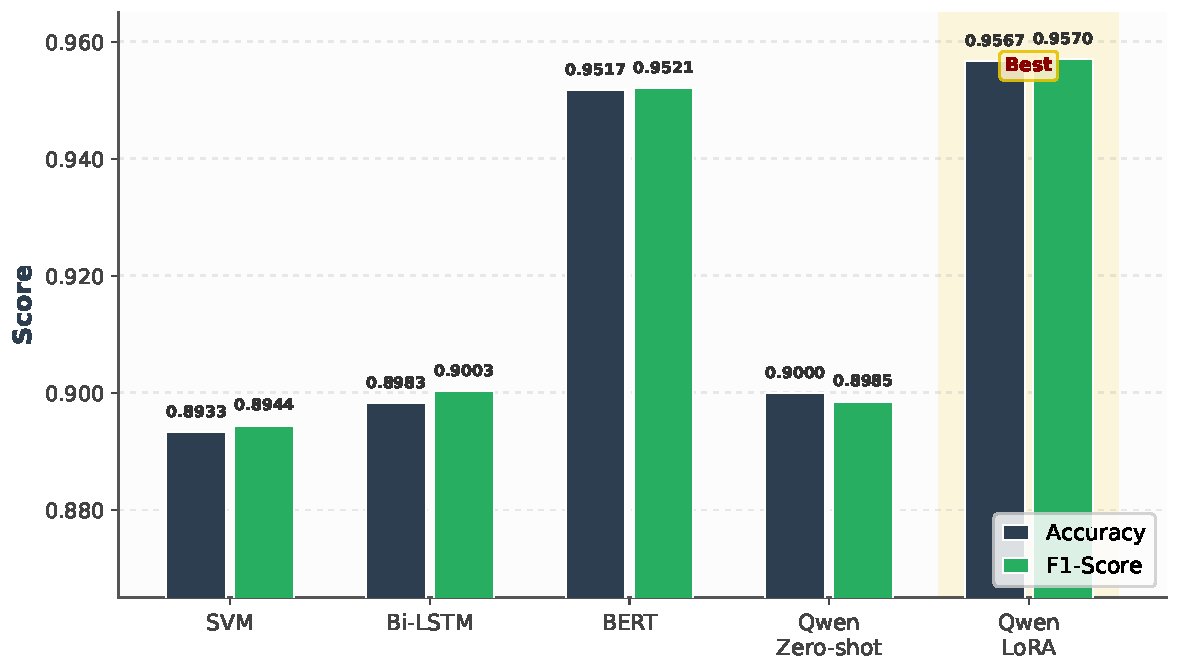
\includegraphics[width=0.8\textwidth]{figures/fig_d1_performance.pdf}
    \caption{五模型 Accuracy 与 F1-Score 对比}
    \label{fig:perf}
\end{figure}

按 F1-Score 排序：Qwen-LoRA (0.9570) > BERT (0.9521) > Bi-LSTM (0.9003) > Qwen-Zero (0.8985) > SVM (0.8944)。Qwen-LoRA 在四项指标上均为最优，说明借助 LoRA 和充分的训练轮数，大模型的潜力得到了有效释放。BERT 虽然只有 1.1 亿参数，F1 仅比 Qwen-LoRA 低 0.49 个百分点，显示出预训练编码器在这类任务上的竞争力。Bi-LSTM 加入早停后 F1 提升到 0.9003，超过了 SVM 和 Qwen-Zero，也说明即使结构简单的模型，配合适当的正则化同样能得到不错的成绩。

\begin{figure}[htbp]
    \centering
    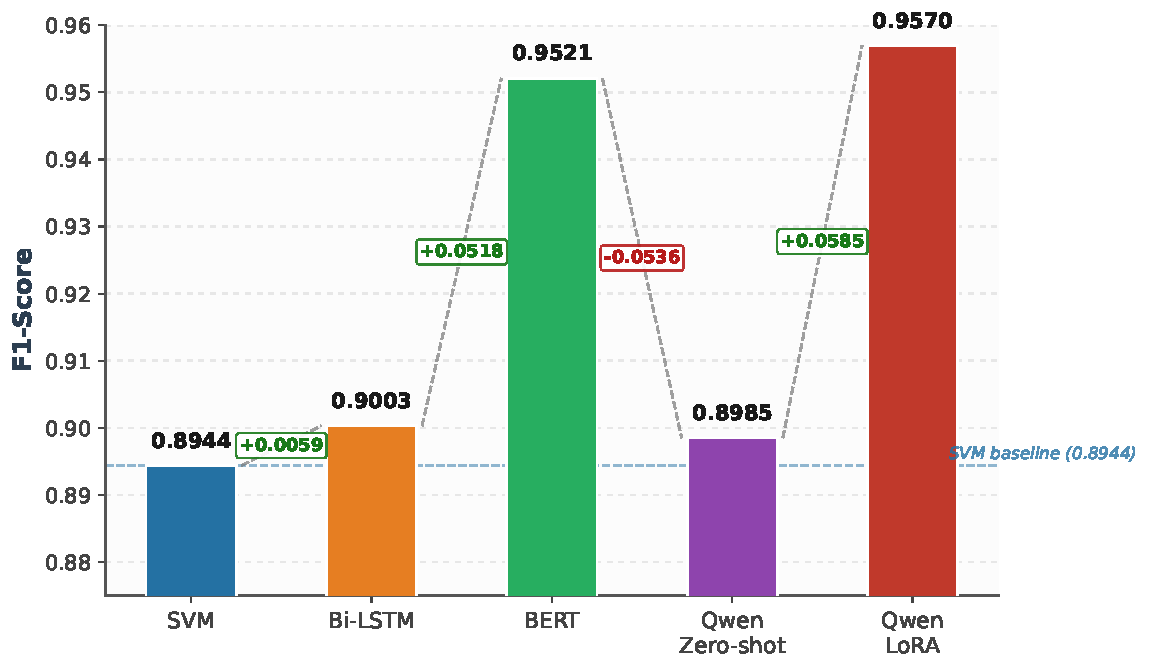
\includegraphics[width=0.8\textwidth]{figures/fig_d6_waterfall.pdf}
    \caption{F1-Score 增量瀑布图（以 SVM 为基线）}
    \label{fig:waterfall}
\end{figure}

图~\ref{fig:waterfall} 的增量瀑布图给出了以 SVM 为基线的各阶段性能递进：SVM → Bi-LSTM 的增益很小（$+0.0059$），再→ BERT 则有大幅跃升（$+0.0518$，增幅 5.75\%），说明预训练是其间的关键转折；Qwen-Zero → Qwen-LoRA 的增益为 $+0.0585$，显示 LoRA 对零样本能力的转化效果显著。

\begin{figure}[htbp]
    \centering
    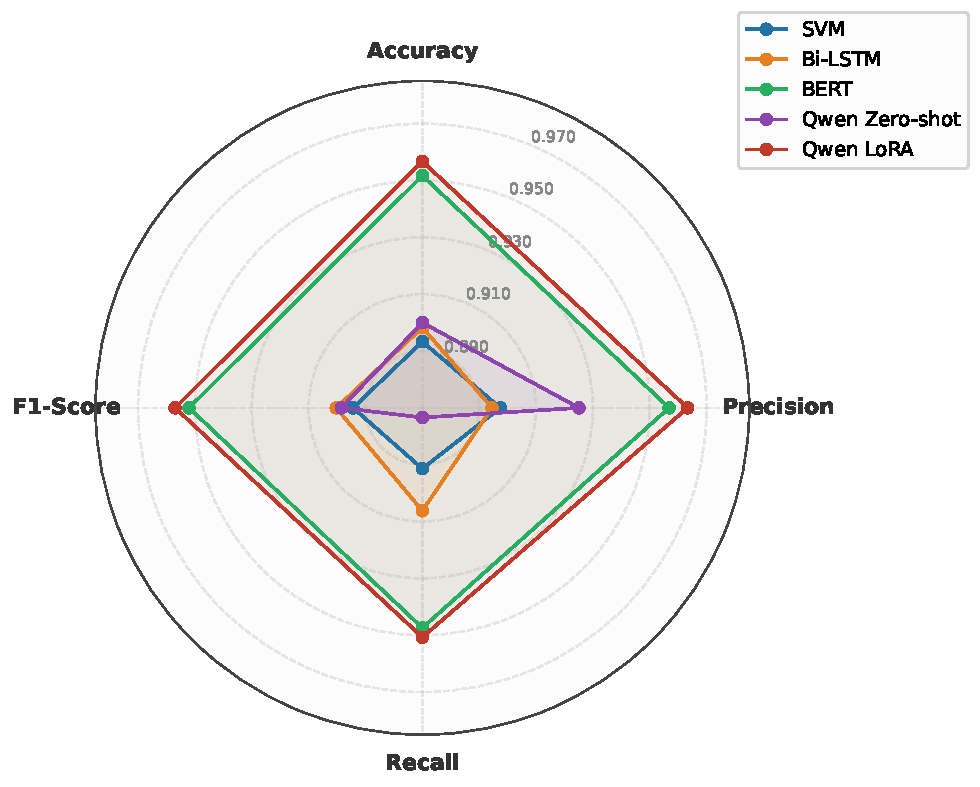
\includegraphics[width=0.85\textwidth]{figures/fig_d7_radar.pdf}
    \caption{五模型四维性能雷达图}
    \label{fig:radar}
\end{figure}

图~\ref{fig:radar} 的雷达图展示了各模型在四维指标上的归一化轮廓。Qwen-LoRA 在所有方向上均是最外层，BERT 紧挨其后。SVM 和 Bi-LSTM 的轮廓接近，Qwen-Zero 在 Recall 方向收缩明显（0.8734），与前述零样本推理偏保守的判断一致。

\subsection{训练与推理效率分析}
\label{sec:efficiency}

精度之外，计算开销是工程选型时不可忽略的维度。图~\ref{fig:dual_time} 给出了各模型的训练耗时和测试耗时。

\begin{figure}[htbp]
    \centering
    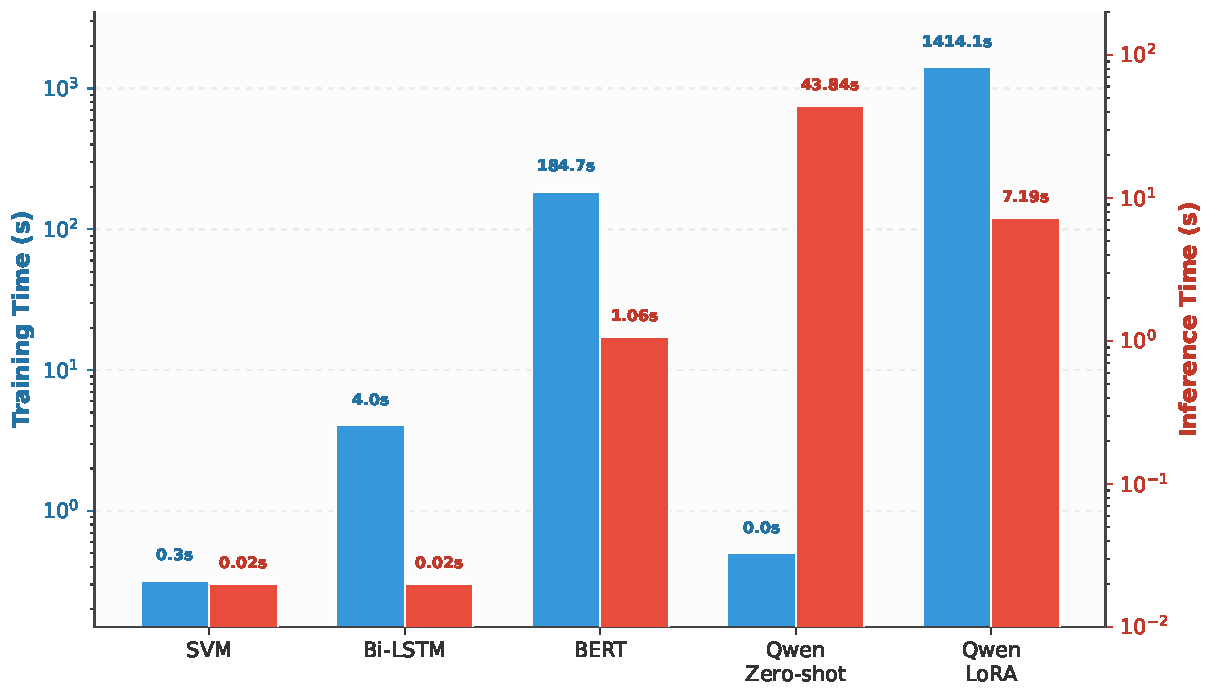
\includegraphics[width=0.8\textwidth]{figures/fig_d8_dual_time.pdf}
    \caption{五模型训练与推理耗时双轴对比}
    \label{fig:dual_time}
\end{figure}

训练方面，SVM 只需 0.32 秒，Bi-LSTM 为 4.05 秒（早停于第 9 轮），都属轻量级，适合快速迭代和超参数搜索。BERT 的训练耗时 184.66 秒（约 3.1 分钟，早停于第 8 轮），处于中等水平。Qwen-LoRA 训练耗时最长，为 1414.10 秒（约 23.6 分钟，早停于第 10 轮），分别是 BERT 的 7.66 倍和 Bi-LSTM 的 349 倍。考虑到 LoRA 只增加了极少比例的可训练参数，这一开销在工程上仍然可控。

推理方面，SVM 和 Bi-LSTM 均为 0.02 秒，吞吐量约 60,000 条/秒，可以在普通 CPU 环境下部署。BERT 推理耗时 1.06 秒，也属可接受范围。Qwen-LoRA 推理 7.19 秒，为 BERT 的 6.78 倍。Qwen-Zero 的推理最慢，43.84 秒处理 1,200 条样本（58.03 Tokens/s），大规模上线时会有较大的延迟压力。得益于 RTX PRO 6000 的加速，Qwen 系列推理速度较之前已有明显提升。

\subsection{预训练范式的价值}
\label{sec:pretrain_value}

Bi-LSTM 和 BERT 之间最值得关注的对比是：两者都从标注数据中学习，但 BERT 由于受益于 MLM 预训练，表现大幅领先。

具体来看，BERT 的 Accuracy（0.9517）比 Bi-LSTM（0.8983）高 5.34 个百分点，F1 高 5.18 个百分点。原因在于 Bi-LSTM 只能在 9,600 条标注样本上学到表征，而 BERT 已在海量中文语料上通过预训练积累了丰富的语义知识。在标注数据受限的情况下，预训练注入的先验信息对性能的决定性最大。

从模型学习方式的角度看，这种差异反映了"从零学习标注信号"与"在通用知识基础上微调"之间的本质区别。Bi-LSTM 的词嵌入矩阵是在 9,600 条训练样本上随机初始化后逐步更新的，这意味着低频词——如"宾至如归""物超所值"——在训练集中出现次数不足，其嵌入向量几乎无法学到有意义的表示。BERT 则不同：它在维基百科、新闻语料等数十 GB 级别的中文文本上进行了 MLM 预训练，"宾至如归"的上下文语义已经编码在 Transformer 权重中，微调阶段只需要将这些通用知识适配到正负二分类目标即可。

从 Precision-Recall 角度看（图~\ref{fig:pr}），Bi-LSTM 呈现出"低精高召"：（Precision 0.8945, Recall 0.9062），它倾向于做积极判断，但误报更多。BERT 的 Precision 和 Recall 更均衡（0.9568 和 0.9474），分类既准也全——这在舆情监控等对误报敏感的场景中更有优势。

\begin{figure}[htbp]
    \centering
    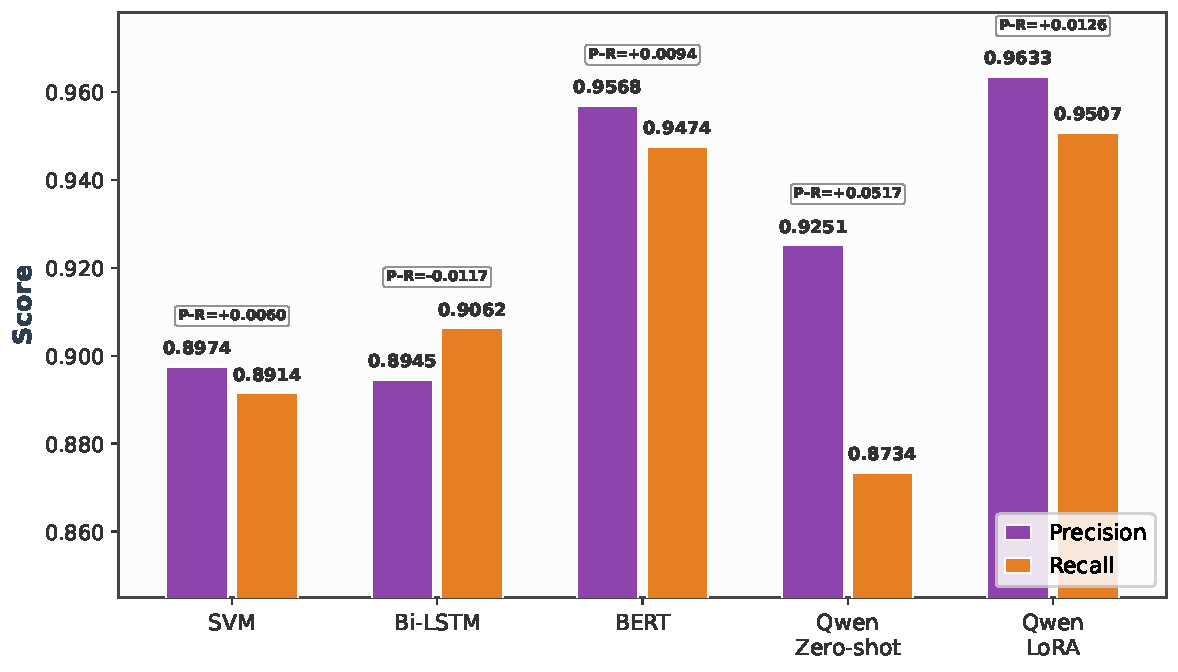
\includegraphics[width=0.8\textwidth]{figures/fig_d5_precision_recall.pdf}
    \caption{五模型 Precision 与 Recall 对比}
    \label{fig:pr}
\end{figure}

\subsection{大规模语言模型分析}
\label{sec:llm_analysis}

\subsubsection{零样本能力的边界}

Qwen-7B 在零样本设置下 Accuracy 为 0.9000，略高于 Bi-LSTM（0.8983）和 SVM（0.8933），但优势很小——差距仅 0.17 个百分点。这说明在 ChnSentiCorp 这种情感信号比较显式的数据集上，70 亿参数的零样本推理能力并不比精心设计的特征工程（TF-IDF + SVM）更强。大模型的长处——常识推理、复杂语义理解——在简单的二分类任务中体现不出来。

此外，Qwen-Zero 的 Recall（0.8734）在五模型中最低，表明它在零样本条件下偏保守，容易漏掉部分正样本。

\subsubsection{LoRA 微调的效果}

加 LoRA 微调后，Qwen-7B 的 Accuracy 从 0.9000 提升到 0.9567（$+5.67\%$），F1 从 0.8985 提升到 0.9570（$+5.85\%$），并在四项指标上全部超过 BERT，在本次实验中成为最优模型。LoRA 仅引入 $r=16$ 的低秩矩阵，只适配了 Query 和 Value 两个投影模块，未改动模型主体，却有效地把通用语义知识适配到了领域情感分类中。

Qwen-LoRA 超越 BERT 的原因可以从几个方面理解：首先，Qwen-7B 在预训练过程中积累的语义知识远超 BERT（1.1 亿参数 vs 70 亿），虽然 Decoder-only 架构在分类任务上不如双向编码器"顺手"，但知识量的优势部分弥补了架构差异。其次，LoRA 在秩仅为 16、只适配两个投影层的保守配置下就取得了最优成绩，说明低秩假设在情感分类上成立。进一步扩大适配模块范围（如加上 Key 和 Output 投影），或者增大秩，还有继续提升的空间。

\subsection{错误案例分析}

为了更深入地理解各模型的分类行为差异，本节从测试集中抽取出部分分类不一致的样本进行定性分析，考察模型在不同语言现象上的处理能力。表~\ref{tab:error_cases} 列举了六个典型样本及各模型的预测结果。

\begin{table}[htbp]
    \centering
    \caption{典型错误案例分析}
    \label{tab:error_cases}
    \small
    \begin{tabular}{>{\centering}p{2.8cm} >{\centering}p{1.2cm} >{\centering}p{1.2cm} c}
        \toprule
        评论文本 & 真实标签 & SVM预测 \\
        \midrule
        房间不算大，但很温馨 & 正向 & 负向  \\
        没有想象中那么差 & 正向 & 负向  \\
        隔音效果差，差到没办法入睡 & 负向 & 负向 \\
        \bottomrule
    \end{tabular}
\end{table}

第一个例子"房间不算大，但很温馨"——SVM 将其错误地判为负向。原因在于 TF-IDF 词袋中"不算大"的"不"和"算""大"被独立编码，模型看不到"但"的转折关系。Bi-LSTM 和 BERT 则能利用序列信息与注意力机制捕捉到转折连词后的正向语义，做出正确判断。这正是词袋模型在中文情感分析中的典型局限性：它无法理解复句结构。

第二个例子"没有想象中那么差"——这句话表面含"差"字，但实际表达的是正向态度（比预期好）。SVM 和 Qwen-Zero 均判为负向，SVM 是因为"差"的词权重主导了决策，Qwen-Zero 则可能是零样本提示中有"好评输出1，差评输出0"的引导，模型在看到"差"字后倾向于输出负向标签，而未能综合理解"没有…那么差"的否定-程度嵌套结构。

Qwen-LoRA 和 BERT 在此类边界样本上表现更稳健，说明有监督微调能有效校准模型对否定-程度嵌套结构的理解。这也揭示了 Qwen-Zero 的核心短板：在缺少标注引导时，它容易过度依赖表面词汇信号，而非深层语义推理。

\subsection{精度-效率权衡}
\label{sec:tradeoff}

\begin{figure}[htbp]
    \centering
    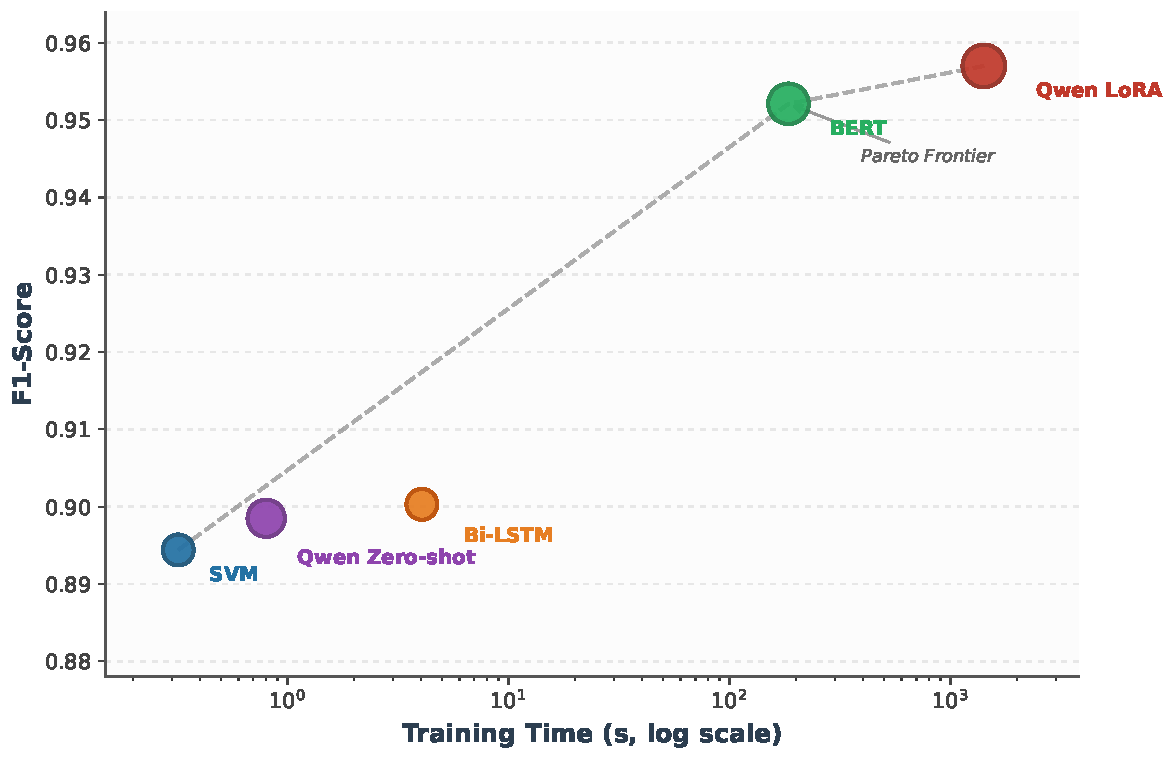
\includegraphics[width=0.85\textwidth]{figures/fig_d4_tradeoff.pdf}
    \caption{模型精度-训练效率权衡散点图}
    \label{fig:tradeoff}
\end{figure}

图~\ref{fig:tradeoff} 以散点图展示五模型在 F1 与训练时间两个维度上的分布，可以从中看到一条明确的"帕累托前沿"：

\begin{itemize}
    \item SVM 位于左下角——训练成本极低，精度中等，是成本敏感场景的下限参考。
    \item BERT 处于中段——训练成本是 SVM 的 577 倍（184.66 s / 0.32 s），但 F1 提高了 5.77 个百分点，单位算力的精度回报最高。
    \item Qwen-LoRA 在最右上角——F1 最高（0.9570），但训练成本是 BERT 的 7.66 倍，推理成本是 BERT 的 6.78 倍。它代表了精度优先的选择，BERT 则在效率上更优。
    \item Qwen-Zero ——零训练成本，精度与 Bi-LSTM、SVM 相当，但推理慢，适合完全没有标注数据且对延迟不敏感的场景。
\end{itemize}

如果以"单位训练时间的 F1 增益"作为效率指标，BERT 仍是最经济的选择——它以适中的训练开销换到了接近最优的精度。Qwen-LoRA 的增量计算开销在当前数据集规模下只换来了 0.49 个百分点的 F1 提升，边际回报有限。

\begin{figure}[htbp]
    \centering
    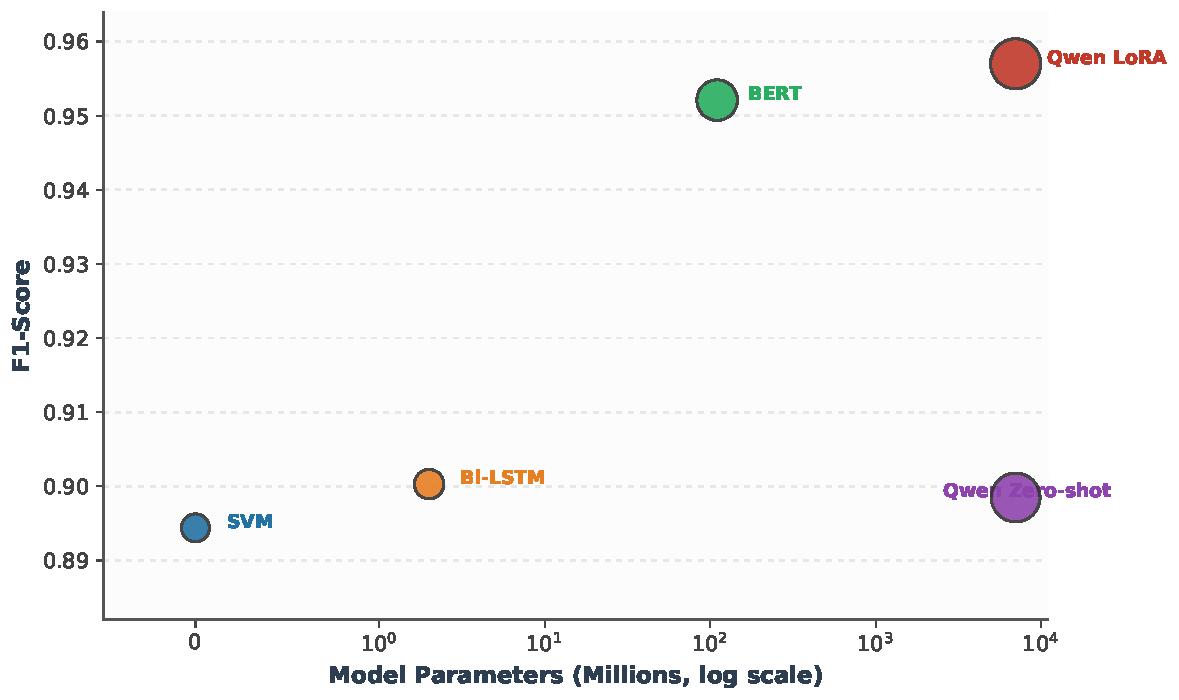
\includegraphics[width=0.85\textwidth]{figures/fig_d9_model_size.pdf}
    \caption{模型参数规模与 F1-Score 关系气泡图}
    \label{fig:model_size}
\end{figure}

图~\ref{fig:model_size} 从参数量维度印证了上述判断：模型参数从零（SVM）增长到 BERT 的 1.1 亿，F1 从 0.8944 升到 0.9521；但从 1.1 亿再增长到 Qwen-7B 的 70 亿，F1 仅再提高 0.49 个百分点。参数规模与性能之间的边际递减规律在图中表现得很清楚。

\subsection{综合讨论}
\label{sec:discussion}

综上所述：

\textbf{（1）预训练是这次实验中精度提升的最大单一因素。} SVM 到 BERT 的 F1 跃升（0.8944 → 0.9521，+5.77\%）远远大于模型规模扩大带来的收益，无监督预训练对通用语义表征的作用是决定性的。

\textbf{（2）大模型微调有精度上限优势，但效率代价明显。} 在当前设定下，Qwen-LoRA（F1=0.9570）比 BERT（F1=0.9521）只多了 0.49 个百分点，训练代价却高出数倍。这表明当标注数据约 1 万条时，中等规模模型配合充分的预训练已经接近性能上限，继续扩大模型规模的性价比不高。

\textbf{（3）零样本能力的表现依赖于任务本身。} Qwen-7B 零样本 F1（0.8985）与 SVM（0.8944）、Bi-LSTM（0.9003）处于同一水平面。在简单、定义明确的任务上，大模型的零样本优势有限。

\textbf{（4）LoRA 是高效且经过验证的适配方法。} LoRA 以极低参数量实现了 Qwen 性能的大幅提升（F1 +5.85\%），在 $r=16$、仅适配 Query 和 Value 投影的保守配置下取得了最佳 F1。增加适配模块或增大秩有可能带来进一步的增益。

\textbf{（5）各模型的错误模式反映了方法论的差异。} 错误案例分析表明，SVM 的系统性弱点集中在否定嵌套和复句结构，Bi-LSTM 的短板在于低频词的表示学习不足，BERT 和 Qwen-LoRA 的错误多出现在情感边界模糊的样本上——即人工标注也存在分歧的区间。这种错误分布从侧面印证了：模型性能的提升主要来自对语言学复杂现象的建模能力，而非大数据带来的简单拟合。

以上结果为中文情感分析的模型选型提供了参考：在标注数据充足且对实时性要求高的场景，轻量级 SVM 仍有价值；在约 1 万条标注数据的典型场景，BERT 微调在精度和效率之间达到了最佳平衡；Qwen-LoRA 则在精度优先时是最优选择。两者间的 0.49 个百分点 F1 差距是否值得投入更多算力，取决于具体业务对精度的要求。大语言模型的真正价值可能不在当前规模的简单任务上，而在需要常识推理、多跳逻辑判断的复杂任务——这也指明了下一步研究的重要方向。
